\documentclass[a4paper]{article}

%% Language and font encodings
\usepackage[english]{babel}
\usepackage[utf8x]{inputenc}
\usepackage[T1]{fontenc}
\usepackage{wrapfig, blindtext}

%% Sets page size and margins
\usepackage[a4paper,top=3cm,bottom=2cm,left=3cm,right=3cm,marginparwidth=1.75cm]{geometry}

%% Useful packages
\usepackage{amsmath}
\usepackage{graphicx}
\usepackage[colorinlistoftodos]{todonotes}
\usepackage[colorlinks=true, allcolors=blue]{hyperref}

%Paquete para utilizar algoritmos
\usepackage[linesnumbered,ruled,vlined]{algorithm2e}
\usepackage{algorithmic}
\pagestyle{myheadings}

%Caratula
\begin{document}
\begin{titlepage}
\begin{center}
\vspace*{-0.4in}

{\fontsize{12}{30}\bf \selectfont UNIVERSIDAD NACIONAL DE INGENIERIA\\}

{\fontsize{12}{40}\bf \selectfont FACULTAD DE CIENCIAS\\}
\vspace*{0.15in} CIENCIAS DE LA COMPUTACI\'ON\\
\vspace*{0.2in}
\begin{figure}[htb]
\begin{center}

\includegraphics[width=4.5cm,height=6.5cm]{UNI.png}
\end{center}
\end{figure}
\begin{Large}
\textbf{INTRODUCCI\'ON A LA INTELIGENCIA ARTIFICIAL\\}
\end{Large}
\vspace*{0.2in}

\begin{large}
{\bf T\'itulo del Trabajo\\}
\vspace*{0.1in}
{\fontsize{12}{13}\selectfont 
Problema de Coloraci\'on de Mapas modelado como\\ Problema de Satisfacci\'on de Restricciones\\}
\end{large}
\vspace*{0.3in}

\begin{large}
{\bf Autores} 
\vspace*{0.1in}
\\L\'azaro Camasca, Edson Nicks\\
Le\'on Rios, Marco Naro \\Inocente Valle, Patrichs\\
V\'ictor Ponce, Pinedo
\end{large}

\vspace*{0.4in}
\begin{large}
{\bf Profesor} 
\vspace*{0.1in}
\\Lara Avila, Cesar
\end{large}

\end{center}
\begin{center}
\begin{large}
\vspace*{1.0in}
Lima - Peru\\
{\bf (2018)}
\end{large}
\end{center}
\end{titlepage}

\pagebreak
\tableofcontents
\pagebreak

\section{Resumen}
\subsection{Inteligencia Artificial}
\subsubsection{Conceptos Generales}
La inteligencia artificial es un área de estudio bastante nueva. El propio término de INTELIGENCIA ARTIFICIAL fue implantado en una conferencia en el año de 1956. Esta área aborda la simulación de procesos de inteligencia humana por parte de máquinas, especialmente sistemas informáticos. Estos procesos incluyen el aprendizaje (la adquisición de información y reglas para el uso de la información), el razonamiento (usando las reglas para llegar a conclusiones aproximadas o definitivas) entre otras.
Durante el transcurso del tiempo han habido muchos científicos que han tratado de proporcionar una definición formal de IA. Muchas de estas definiciones se pueden agrupar mediante 4 enfoques distintos:

\begin{enumerate}
\item Sistemas que piensan como humanos
\item Sistemas que actúan como humanos
\item Sistemas que piensan racionalmente
\item Sistemas que actúan racionalmente
\end{enumerate}
Las bases de la Inteligencia artificial son: Filosofía, Economía, Matemáticas, Neurociencia, Psicología, Computación, Linguística.

\subsubsection*{La Prueba de Turing}
Para poder comprobar si efectivamente un sistema informático es realmente inteligente Alan Turing sugirió una prueba basada en la incapacidad de diferenciar entre entidades inteligentes indiscutibles y seres humanos. Un evaluador humano empieza a formular preguntas a un ser humano y a un sistema informático y estos dos brindarán sus respectivas respuestas. Si el evaluador humano concluye que no puede diferenciar cual de las respuestas provienen del sistema informático entonces se podrá decir que el sistema informático evaluado es inteligente.

\subsubsection*{\'Areas de Aplicaci\'on de IA}
\begin{itemize}
\item Tratamiento de Lenguajes Naturales: capacidad de traducción, órdenes a un sistema operativo, conversación hombre-máquina, etc.
\item Sistemas Expertos: sistemas que se les implementa experiencia para conseguir deducciones cercanas a la realidad.
\item Robótica: navegación de robots móviles, control de brazos móviles, ensamblaje de piezas, etc.
\item Problemas de Percepción: visión y habla, reconocimiento de voz, obtención de fallos por medio de la visión, diagnósticos médicos, etc.
\item Aprendizaje: modelización de conductas para su implante en computadoras.
\end{itemize}

\subsubsection*{B\'usqueda heur\'istica}
Primero definamos lo que es una heurística. Una heurística es un algoritmo diseñado para encontrar la solución más óptima posible de un problema dado, sin embargo puede que si bien una solución se arroja de manera rápida, no se puede demostrar que siempre será así, o bien si la heurística nos devuelve la solución correcta no es posible demostrar que ante otros parámetros siempre devuelva la solución correcta. Las heurísticas están orientadas a reducir la cantidad de búsqueda requerida para encontrar una solución.

Ahora, debido a que muchos problemas y las etapas a seguir para resolverlos se pueden modelar mediante grafos, una búsqueda heurística nos ayudará a encontrar el camino más corto entre un nodo dado y el nodo objetivo que vendría a representar para nosotros la solución del problema. Para ello se definen funciones heurísitcas que representan que tan óptimo es ir hacia un nodo dado y en base a dicha función es que se van tomando las decisiones de que camino recorrer para poder llegar al objetivo.

\subsubsection*{Algoritmo A*}
Este algoritmo es un metodo de solución para hallar el camino de menor coste en un grafo desde un nodo en específo hasta otro. Para lograr este resultado el algoritmo se vale de una función de evaluación de optimalidad f(n) y de funciones g(n) y h(n) donde:
\begin{itemize}
\item f(n): coste más barato estimado de la solución a través de n.
\item g(n): coste del camino desde el nodo inicio al nodo n.
\item h(n): función heurística que determina el coste estimado del camino más barato desde n al objetivo. Lo que hará un algoritmo en un nodo x determinado será analizar mediante la función f los nodos adyacentes a x y el nodo y escogido será el que nos devuelve el menor coste, es decir, el menor f(y) de todos.
\end{itemize}


\subsubsection{B\'usqueda entre Adversarios}
El problema de búsqueda entre adversarios, también conocido como juego. El jugar a juegos fue una de las primeras tareas emprendidas en IA. Desde 1950 hasta la actualidad hubo un progreso continuo en el nivel de juego, hasta el punto de que las máquinas han derrotado a campeones humanos en ajedrez. Los juegos son interesantes porque son demasiado difíciles de resolver. Por ejemplo, el ajedrez tiene un árbol de búsqueda de aproximadamente $10^5$ nodos por lo tanto se requiere la capacidad de tomar decisiones óptimas.
Los juegos en inteligencia artificial, son aquel entorno en donde agentes tendrán que considerar las acciones de otros agentes, los agentes se encuentran en conflicto y ambos jugadores tratan de maximizar su rendimiento. Un juego puede definirse por el estado inicial (como se establece en el tablero), las acciones legales en cada estado, un test terminal (que dice cuándo el juego está terminado), y una función de utilidad que se aplica a los estados terminales.

\subsubsection*{Clasificacion de juegos seg\'un IA:}
\begin{itemize}
\item Juegos de suma cero.
\item Minimax o de dos jugadores.
\item Por turnos.
\item Deterministas.
\item De información perfecta, como por ejemplo el Ajedrez. 
\end{itemize}

En juegos de suma cero de dos jugadores con información perfecta, el algoritmo minimax puede seleccionar movimientos óptimos usando una enumeración primero en profundidad del árbol de juegos.
El algoritmo de búsqueda alfa-beta calcula el mismo movimiento óptimo que el minimax, pero consigue una eficiencia mucho mayor, eliminando subárboles que son probablemente irrelevantes

\subsubsection{Problema de Satisfacci\'on de Restricciones}
El PSR modela los problemas como una colección homogénea finita de restricciones sobre variables, las que son resueltas por métodos de satisfacción de restricciones. Las etapas básicas para la resolución de un problema PSR son su modelización y su posterior resolución mediante la aplicación de técnicas PSR específicas, que incluyen procesos de búsqueda apoyados con métodos heurísticos y procesos inferenciales. El modelamiento del problema, que permite representar un problema mediante un conjunto finito de variables, un dominio de valores finito para cada variable y un conjunto de restricciones que acotan las combinaciones válidas de valores que las variables pueden tomar. En el modelamiento de un PSR, es fundamental la capacidad expresiva, a fin de poder captar todos los aspectos significativos del problema a modelar.
Ejemplos típicos de problemas que se pueden modelar como PSR 
son:
\begin{itemize}
\item El problema de las N reinas
\item La coloración de mapas 
\item Sudoku 
\item Problemas de criptoaritmética
\end{itemize}

\subsubsection{Machine Learning}
Es un tipo de inteligencia artificial (AI) que proporciona a las computadoras la capacidad de aprendizaje automatico, sin ser programadas explícitamente. El aprendizaje automático se centra en el desarrollo de programas informáticos que pueden cambiar cuando se exponen a nuevos datos.

\subsection*{Modelos Lineales}
\subsubsection*{Perceptron}
Es la red de neuronas artificiales más sencilla. Está compuesta únicamente por una capa de neuronas de entrada y otra capa de neuronas de salida. El Perceptrón es una red capaz de aprender. En su configuración inicial a los pesos de las conexiones se les da valores arbitrarios, por lo que ante la presencia de estímulos,la red genera respuestas arbitrarias, respuestas que no coinciden con las deseadas, y no es hasta que los pesos se han ajustado de tal modo que la respuesta que emite es la deseada, que se considera que la red ha conseguido aprender.

\subsubsection*{K-Vecinos m\'as cercanos}
Es un algoritmo clasificador supervisado basado en Reconocimiento de patrones en criterios de vecindad, y también se conoce como algoritmo de clasificación k-NN. Parte de la idea de que una nueva muestra será clasificada a la clase a la cual pertenezca la mayor cantidad de vecinos más cercanos del conjunto de entrenamiento más cercano a ésta.

\subsubsection*{SVM}
Son las siglas de Support Vector Machine. Este algoritmo supervisado se utiliza generalmente para solucionar problemas de clasificación. La idea del algoritmo es ser capaces de encontrar, con los datos de entrenamiento, un hiperplano que maximiza la distancia a las diferentes clases, lo que es conocido como el “margen máximo”.
Una vez hallado este hiperplano podemos usarlo para clasificar nuevos puntos.
SVM tiene múltiples aplicaciones, por ejemplo para reconocimiento de imágenes, clasificación de texto o aplicaciones en el área de la biotecnología.

\subsubsection*{Arboles de decisión}
Es una forma gráfica y analítica de representar todos los eventos (sucesos) que
pueden surgir a partir de una decisión asumida en cierto momento. Nos ayudan a tomar la decisión “más acertada”, desde un punto de vista probabilístico, ante un
abanico de posibles decisiones.

\subsubsection*{Redes Neuronales}
Consisten de unidades de procesamiento que intercambian datos o
información,se utilizan para reconocer patrones, incluyendo imágenes, manuscritos y
secuencias de tiempo (por ejemplo: tendencias financieras).

Tienen capacidad de aprender y mejorar su funcionamiento. Una primera clasificación de los modelos de redes neuronales podría ser,
atendiendo a su similitud con la realidad biológica:
\begin{itemize}
\item El modelo de tipo biológico. Este comprende las redes que tratan de simular los sistemas neuronales biológicos, así como las funciones auditivas o algunas funciones básicas de la visión.
\item El modelo dirigido a aplicación. Este modelo no tiene por qué guardar similitud con los sistemas biológicos. Su arquitectura está fuertemente ligada a las necesidades de las aplicaciones para la que es diseñada.

\end{itemize}

\subsubsection{Proceso de Markov}
Un proceso de Markov es un tipo especial de proceso estocástico que describe la evolución de un sistema de variables aleatorias con la particularidad de que la valor de la probabilidad de un estado depende solamente del valor de la probabilidad del estado anterior.

Mas formalmente, para el caso discreto:
Un proceso de Markov, usualmente llamado Cadena de Markov, está definido por:
Un conjunto de estado $\ S = \{1,..., n\}$
Un conjunto de posibles transiciones, a saber, los pares $(i, j)$ para los cuales $p_{ij} > 0$, y, los valores numéricos para los cuales $p_{ij}$ son positivos.\\
El proceso de Markov definido por una colección de variables aleatorias $X_{0},\\
X_{1},...,X_{n},...,$ que toman valores de $S$ y que satisfacen $\ P(X_{n+1} = j | X_{n} = i, X_{n-1} = i_{n-1},..., X_{0} = i_{0}) = p_{ij}$

Para los estados $i,j \in S$ y las posibles secuenvias $i_{0},..., i_{n+1}$ de esos estados.

El rango de aplicación del modelo de Markov es extenso. Uno de ellos es el aprendizaje por reforzamiento

\subsubsection*{Aprendizaje por reforzamiento}
Área del Machine Learning que toma ideas del conductismo en las cuales se determina las acciones que debe escoger un programa para obtener el mayor estimulo positivo de parte del entorno.

La situación donde el "estimulo" del ambiente depende, en una cierta medida mas no en toda, de las acciones que el agente realiza en el estado anterior puede modelarse mediante un proceso estocástico de Markov debido a que la respuesta del ambiente depende, en cierta medida, de las acciones del agente.


\textbf{
Dentro de todos los temas mencionados anteriormente se escogio el PROBLEMA DE SATISFACCIÓN DE RESTRICCIONES}
% 
%\subsection{Breve descripción del problema}
%\subsection{Resumen de lo realizado en R}
%\subsection{Breve descripci\'on de las prubeas realizadas}
%\subsection{Resumen de la concluci\'on}



\section{Introducci\'on}
\subsection{Definición de un  Problema de Satisfacción de Restriciones}
Un promebla de satisfacción de restricciones(o PSR) está definido por:
\begin{itemize}
	\item Un conjunto de \textbf{variables}, $\{X_1, X_2,..., X_n\}$
	\item Un conjunto de \textbf{dominios}, $\{D_1, D_2,..., D_n\}$
	\item Un conjunto de \textbf{restricciones}, $\{C_1, C_2,..., C_n\}$
\end{itemize} 
A cada variable $X_i$ le corresponde un dominio no vacio $D_i$, los dominios son los valores posibles que puede tomar la variable. 

\textbf{Estado}\\ 
Un estado se define como una asignación de valores a una o todas las variables, $\{X_i = v_i, X_j = v_j...\}$. A un estado que no viole ninguna restricción se le llama estado \textbf{consistente}. Un estado \textbf{completo} es una asignacion en que se menciona cada variable, es decir que se asigne valores a todas las variables.

\textbf{Solución a un PSR}\\
Es un estado completo y consistente. Es decir, es la asignación de valores a todas las variables de tal forma que satisfagan todas las restricción.

\subsection{Problema de Coloración de Mapas}
Dentro del Problema de Satisfacción de Restricciones se escogio el problema de coloración de mapas.\\
El problema de coloración de mapas es un problema que se puede modelar como un PSR.
\subsubsection*{Definicion}
El Problema de coloración de mapas es aquel problema donde se tiene un \textbf{conjunto de colores} y un \textbf{mapa plano} dividido en regiones. El objetivo es colorear cada región del mapa de manera que regiones adyacentes\textbf{(frontera)} tengan distintos colores.

\subsection{Teorema de los 4 Colores}
El teorema menciona que basta solo 4 colores para colorear cualquier \textbf{mapa geográfico plano}, de modo que dos regiones con \textbf{frontera} común tengan diferente color. Además existen condiciones como:
\begin{itemize}
\item El mapa debe ser \textbf{conexo} y cada una de las regiones también es conexa.
\item Se considera frontera, cuando dos regiones se tocan en mas de un punto.
\end{itemize}

\subsection{Resolución del PSR}
La resolución de un Problema de Satisfacción de Restricciones consta de dos fases, que son:

\subsubsection{Modelazión del Problema}
La modelazión de un problema es una parte muy importante para la resolución de problemas, el modelado se realizara en términos de \textbf{variables}, \textbf{dominios} y \textbf{restricciones}.

Gracias al modelamiento del Problema de coloración de mapas como un problema de PSR, se podra demostrar el Teorema de los Colores con ayuda de un ordenador.\\ 

La forma de modelar el problema dentro del PSR es asociando lo siguiente:
\begin{itemize}
\item Una \textbf{variable} $X_i$ por cada región del mapa.
\item El \textbf{dominio} $D_i$ sea el conjunto de colores disponibles.
\item Una \textbf{restricción} $C_i$ para cada par de regiones contiguas sobre la variable correspondiente que no permita la asignación de identicos valores a las variables.
\end{itemize}

Para una mejor ilustracion, supongamos que tenemos un mapa con 8 regiones  $\{r_1, r_2,..., r_8\}$, donde cada region $r_i$ es adyacente a la region $r_{i+1}$ donde $i = \{1,..,8\}$, además las regiones deben ser coloreadas con los posibles colores Rojo, Azul, Negro. La modelacion PSR sería:
\begin{itemize}
\item Variables: $\{r_1 = v_1, r_2 = v_1,..., r_8 = v_8\}$
\item Dominio: $\{Rojo, Azul, Negro\}$, un color para cada variable.
\item Restricciones: $\{r_i \not= r_{i+1}\}$
\end{itemize}

Para la demostración de el teorema de los cuatro colores se utilizara un \textbf{dominio} que contenga solo cuatro colores.




\subsubsection{Procesar las restricciones}
Una vez que hemos modelado el problema como un PSR, hay dos formas de procesar las restriccones:

\begin{itemize}
	 
\item \textbf{Técnicas de consistencia}: basadas en la eliminación de valores inconsistentes de los dominios de las variables (es decir, que no verifican las restricciones impuestas).
\item \textbf{Algoritmos de búsqueda}: se basan en la exploración sistemática del espacio de soluciones hasta encontrar una solución (o probar que no existe tal solución en caso contrario) que verifica todas las restricciones del problema.
\end{itemize}

Para la demostración del teorema de los cuatro colores se opto por utilizar Algoritmos de búsqueda, especificamente El Árbol de Búsqueda y Backtraking Cronológico.

\subsubsection*{El Árbol de Búsqueda}

Las posibles combinaciones de la asignación de valores a las variables en un PSR genera un espacio de búsqueda al que se puede dotar de estructura para ser visto como un \textbf{árbol de búsqueda}. De esta forma, después podremos recorrerlo siguiendo la estrategia que queramos. La búsqueda mediante \textbf{backtracking}, que es la base sobre la que se soportan la mayoría de algoritmos para PSR, corresponde a la tradicional exploración en profundidad DFS en el árbol de búsqueda.

La forma más habitual de darle estructura de árbol pasa por asumir que el orden de las variables es estático y no cambia durante la búsqueda, y entonces un nodo en el nivel k
del árbol de búsqueda representará un estado donde las variables $\{x_1,...,x_k\}$ están asignadas a valores concretos de sus dominios mientras que el resto de variables, $\{x_{k+1},...,x_n\}$, no lo están. Podemos asignar cada nodo en el árbol de búsqueda con la tupla formada por las asignaciones llevadas a cabo hasta ese momento, donde la raíz del árbol de búsqueda representa la tupla vacía, donde ninguna variable tiene asignado valor alguno.\\
%Los nodos del arbol, representan el estado en el codigo R representa el vector color y que los dominios son los colores (1,2,3,4) el color 0 representa que no esta asignado un valor a la variable.%
 
\begin{wrapfigure}{r}{0.5\linewidth}
	\centering
	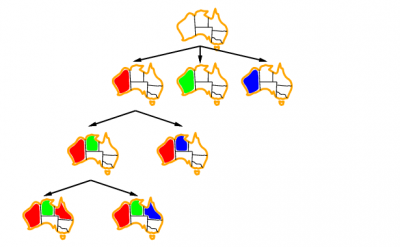
\includegraphics[width=6.5cm,height=5.5cm]{psr-tree.png}
	\caption{Árbol de búsqueda}
	\label{fig:myfig}
\end{wrapfigure}


Los nodos en el primer nivel son 1−tuplas que representan estados donde se les ha asignado un valor a la variable $x_1$. Los nodos en el segundo nivel son 2−tuplas que representan estados donde se le asignan valores a las variables $x_1$ y $x_2$, y así sucesivamente. Un nodo del nivel k es hijo de un nodo del nivel k−1 si la tupla asociada al hijo es una extensión de la de su padre añadiendo una asignación para la variable $x_k$. Si n es el número de variables del problema, los nodos en el nivel n, que representan las hojas del árbol de búsqueda, son n−tuplas, que representan la asignación de valores para todas las variables del problema. De esta manera, si una n−tupla es consistente, entonces es solución del problema.

%En el codigo R se puede a un nodo como el vector color = (0,0,0,.....,0)  representa el el nivel 1 mientras que  los nodos color = (1,0,....,0) , color = (2,0,....,0), color=(3,0,....,0) representan el niver 2, los numeros son los colores que se le asigna a las regiones.%

\subsubsection*{Backtracking Cronológico}

El algoritmo de búsqueda sistemática más conocido para resolver PSR se denomina Algoritmo de Backtracking Cronológico (BT). Si asumimos un orden estático de las variables y de los valores en las variables, este algoritmo funciona de la siguiente manera:

Selecciona la siguiente variable de acuerdo al orden de las variables y le asigna su próximo valor. 
Esta asignación de la variable se comprueba en todas las restricciones en las que forma parte la variable actual y las anteriores:
Si todas las restricciones se han satisfecho, vuelve al punto 1.
Si alguna restricción no se satisface, entonces la asignación actual se deshace y se prueba con el próximo valor de la variable actual. 
Si no se encuentra ningún valor consistente entonces tenemos una situación sin salida (dead-end) y el algoritmo retrocede a la variable anteriormente asignada y prueba asignándole un nuevo valor.
Si asumimos que estamos buscando una sola solución, BT finaliza cuando a todas las variables se les ha asignado un valor, en cuyo caso devuelve una solución, o cuando todas las combinaciones de variable-valor se han probado sin éxito, en cuyo caso no existe solución.

Es fácil generalizar BT a restricciones no binarias. Cuando se prueba un valor de la variable actual, el algoritmo comprobará todas las restricciones en las que sólo forman parte la variable actual y las anteriores. Si una restricción involucra a la variable actual y al menos una variable futura, entonces esta restricción no se comprobará hasta que se hayan asignado todas las variables futuras de la restricción.

BT es un algoritmo muy simple pero muy ineficiente. El problema es que tiene una visión local del problema. Sólo comprueba restricciones que están formadas por la variable actual y las pasadas, e ignora la relación entre la variable actual y las futuras. Además, este algoritmo es ingenuo en el sentido de que no recuerda las acciones previas, y como resultado, puede repetir la misma acción varias veces innecesariamente. Para ayudar a combatir este problema, se han desarrollado algunos algoritmos de búsqueda más robustos.

 

\section{Estado del arte}


\pagebreak
\section{Diseño del experimento}

Para solucionar el coloreo de mapas implementamos el algoritmo del backtraking cronologico:

%usando algoritmos
\begin{algorithm}
	%Etiqueta algoritmo 	
	\caption{Algoritmo de Backtracking Cronológico\label{ALG1_3}}
	\KwIn{Vector de colores V}
	\KwOut{Vector de colores V que satisface PSR}
	Procedimiento $Backtracking(k, V [n])$ \# Llamada inicial: $Backtracking(1, V [n])$ \\
	\hspace{0.1cm} \textbf{Inicio}\\
	\hspace{0.1cm} V [$k$] = $Seleccion(d_k)$\hspace{1cm}\# Selecciona un valor de $d_k$ para asignar a $x_k$ \\
	\hspace{0.1cm} \textbf{si} $Comprobar(k, V [n])$ \textbf{entonces}\\
	\hspace{0.6cm} \textbf{si} $k = n$ \textbf{entonces}\\
	\hspace{1.1cm} \textbf{devolver} $V [n]$\hspace{1cm}\# Es una solución\\
	\hspace{0.6cm} \textbf{sino}\\
	\hspace{1.1cm} $Backtraking(k + 1, V [n])$\\
	\hspace{0.6cm} \textbf{fin si}\\
	\hspace{0.1cm} \textbf{sino}\\
	\hspace{0.6cm} \textbf{si} $quedan valores(dk)$ \textbf{entonces}\\
	\hspace{1.1cm} $Backtraking(k, V [n])$\\
	\hspace{0.6cm} \textbf{sino}\\
	\hspace{1.1cm} \textbf{si} $k = 1$ \textbf{entonces}\\
	\hspace{1.6cm} \textbf{devolver} $\oslash$\hspace{1cm}\# Fallo\\
	\hspace{1.1cm} \textbf{sino}\\
	\hspace{1.6cm} $Backtraking(k - 1, V [n])$\\
	\hspace{1.1cm} \textbf{fin si}\\
	\hspace{0.6cm} \textbf{fin si}\\
	\hspace{0.1cm} \textbf{fin si}\\
	\hspace{0.1cm}\textbf{fin} $Backtraking$
\end{algorithm}



\section{Experimentos y resultados}

\section{Discusi\'on}

\section{Conclusi\'on}

\section{Bibliograf\'ia}
\end{document}